\documentclass[xcolor=dvipsnames, 14pt]{beamer}
%\documentclass[xcolor=dvipsnames, bigger, aspectratio=169]{beamer}

\definecolor{Saffron}{HTML}{F4C430}
\usecolortheme[named=Saffron]{structure}

\mode<presentation> {
	\usetheme[height=2em]{Rochester}
	\setbeamercovered{transparent}
}

\setbeamertemplate{caption}{\insertcaption\par}
\setbeamertemplate{navigation symbols}{}%remove navigation symbols

\setbeamercolor{frametitle}{fg=black}
\setbeamercolor{title}{fg=black}
\setbeamercolor{navigation symbols dimmed}{fg=black!10}
\setbeamercolor{navigation symbols}{fg=black!30}
\setbeamercolor{section number projected}{fg=black}
\setbeamercolor{item projected}{fg=black}


\usepackage[utf8x]{inputenc}
\usepackage[resetfonts]{cmap}
\usepackage{lmodern}
\usepackage[czech,english]{babel}
\usepackage[T1]{fontenc}

\usepackage{graphicx}
\usepackage{amsmath}
\usepackage{amssymb}
\usepackage{listings}
\usepackage{microtype}
\usepackage{tikz}

\usepackage{hyperref}
\hypersetup{unicode=true}

% ----- macros -----
\newcommand{\imageW}[1]{%
  \makebox[\textwidth][c]{\includegraphics[width=1.12\textwidth]{img/#1}}}
\newcommand{\imageH}[1]{%
  \makebox[\textwidth][c]{\includegraphics[height=0.97\textheight]{img/#1}}}

% ---- info -----
\title{Adaptive Learning of Programming}
\author{Jaroslav~Čechák \and Tomáš~Effenberger \and Matěj~Vaněk \and Barbora Vrzáková}
\institute{Faculty of Informatics, Masaryk University}
\date{May 26, 2017}

\begin{document}

\begin{frame}
\titlepage
\end{frame}

\begin{frame}
\frametitle{Mission}
\begin{itemize}
\item app for efficient learning of programming  % (what) ... elementary programming, for kids
\item entertaining problems of optimal difficulty  % (how); ... this lead to
\item max \emph{flow} $\rightarrow$ max efficiency % and happiness as well (why)
\end{itemize}
\end{frame}

\begin{frame}
\frametitle{First Prototype (2016)}
\imageW{first-prototype.png}
% first prototype - for testing our initial ideas and find what works and what not
% - one year of development
% - threw away
% - 50 tasks with a robot in maze
\end{frame}


\begin{frame}
\frametitle{Year of Refactoring}
% what we have worked on whole last year
% it was a big mistake (and useful lesson) to do all large changes in parallel
\begin{itemize}
\item back-end refactoring: clean core, rest API
  % "functional core", "imperative shell" (Django REST)
  % why:
  % - more flexible, e.g. sharing code between web and analyses
  % - easier to understand and hence to debug or extend
  % - better test coverage
  % - systematic collection of all actions
\item front-end: ES6, React, Redux, Material % Design
  % previously: Angular + Bootstrap
  % why: more flexible and understandable, easier development and bug fixing
\item new game: rocket in space
  % different theme, mechanics, graphics
  % why:
  % - the original theme was not flexible and did not allow for a lot of diverse easy tasks,
  %   which is crucial for adaptive learning system
  % - unnecessarily long programs for simple ideas (non-elegant programs)
  % - non-elegant tasks
  % - ugly worlds
  % - not very original and entertaining for kids
  % related changes:
  % - new programming language (RoboCode)
  %   + transformations (ast <-> RoboCode, MiniRoboCode, Blockly, JS)
  % - task source in human-readable/editable markdown (+ task editor)
\item intuitive user interface
  % with cooperation with Bara
  % we have done some changes for more intuitive user interface
  % e.g. mini-instructions
  % still work in progress
\end{itemize}
\end{frame}

\begin{frame}
\frametitle{RoboMission}
\imageW{space-and-blockly.png}
\end{frame}

\begin{frame}
\frametitle{Game Elements}
\imageW{advanced-elements.png}
% asteroids, small shootable meteoroids, colors, wormholes + diamonds
% limits (program length, energy)
% blocks (+ position testing, if-else)
\end{frame}

\begin{frame}
\frametitle{Mini Instructions}
\imageW{mini-instruction.png}
% one time instructions
\end{frame}

%\begin{frame}
%\frametitle{Mini Explanations}
%\imageW{mini-instruction-3.png}
%% "explanations" coupled with a reset action
%\end{frame}

\begin{frame}
\frametitle{Motivation}
\imageW{levels-credits.png}
% simple (external) motivation scheme: credits -> levels
% (but we mostly rely on intrinsic motivation
%   endorsed/promoted by entertaining tasks of optimal difficulty)
\end{frame}

\begin{frame}
\frametitle{Tasks Overview}
\imageW{tasks-overview.png}
% ~ 60 tasks on 9 levels (levels ~ how many blocks available)
\end{frame}

\begin{frame}
\frametitle{Task Editor}
\imageW{task-editor.png}
% it's much easier to create new tasks then in first prototype
% and there are some convenient features of the task editor enabled by the
% refactored parts of the project
\end{frame}


\begin{frame}
\frametitle{RoboCode}
\imageW{task-editor-robocode.png}
% we use common roboAST representation which serves as a mediator between different languages
% we need to support (Blockly for kids, RoboCode for writing, MiniRoboCode for logging, JS for running)
\end{frame}

%\begin{frame}
%\frametitle{SpaceWorld VIM-mode Editing}
%\imageW{task-editor-vim.png}
%% note that the source of each task is just a markdown file,
%% so the whole task source can be edited in vim
%% (no, we don't have emacs version, but pull requests are welcomed)
%\end{frame}


\begin{frame}
\frametitle{Physical Version -- InterSoB 2017}
%\imageW{tasks-overview.png}
% physical version of space world and Blockly built for InterSoB 2017
\centering
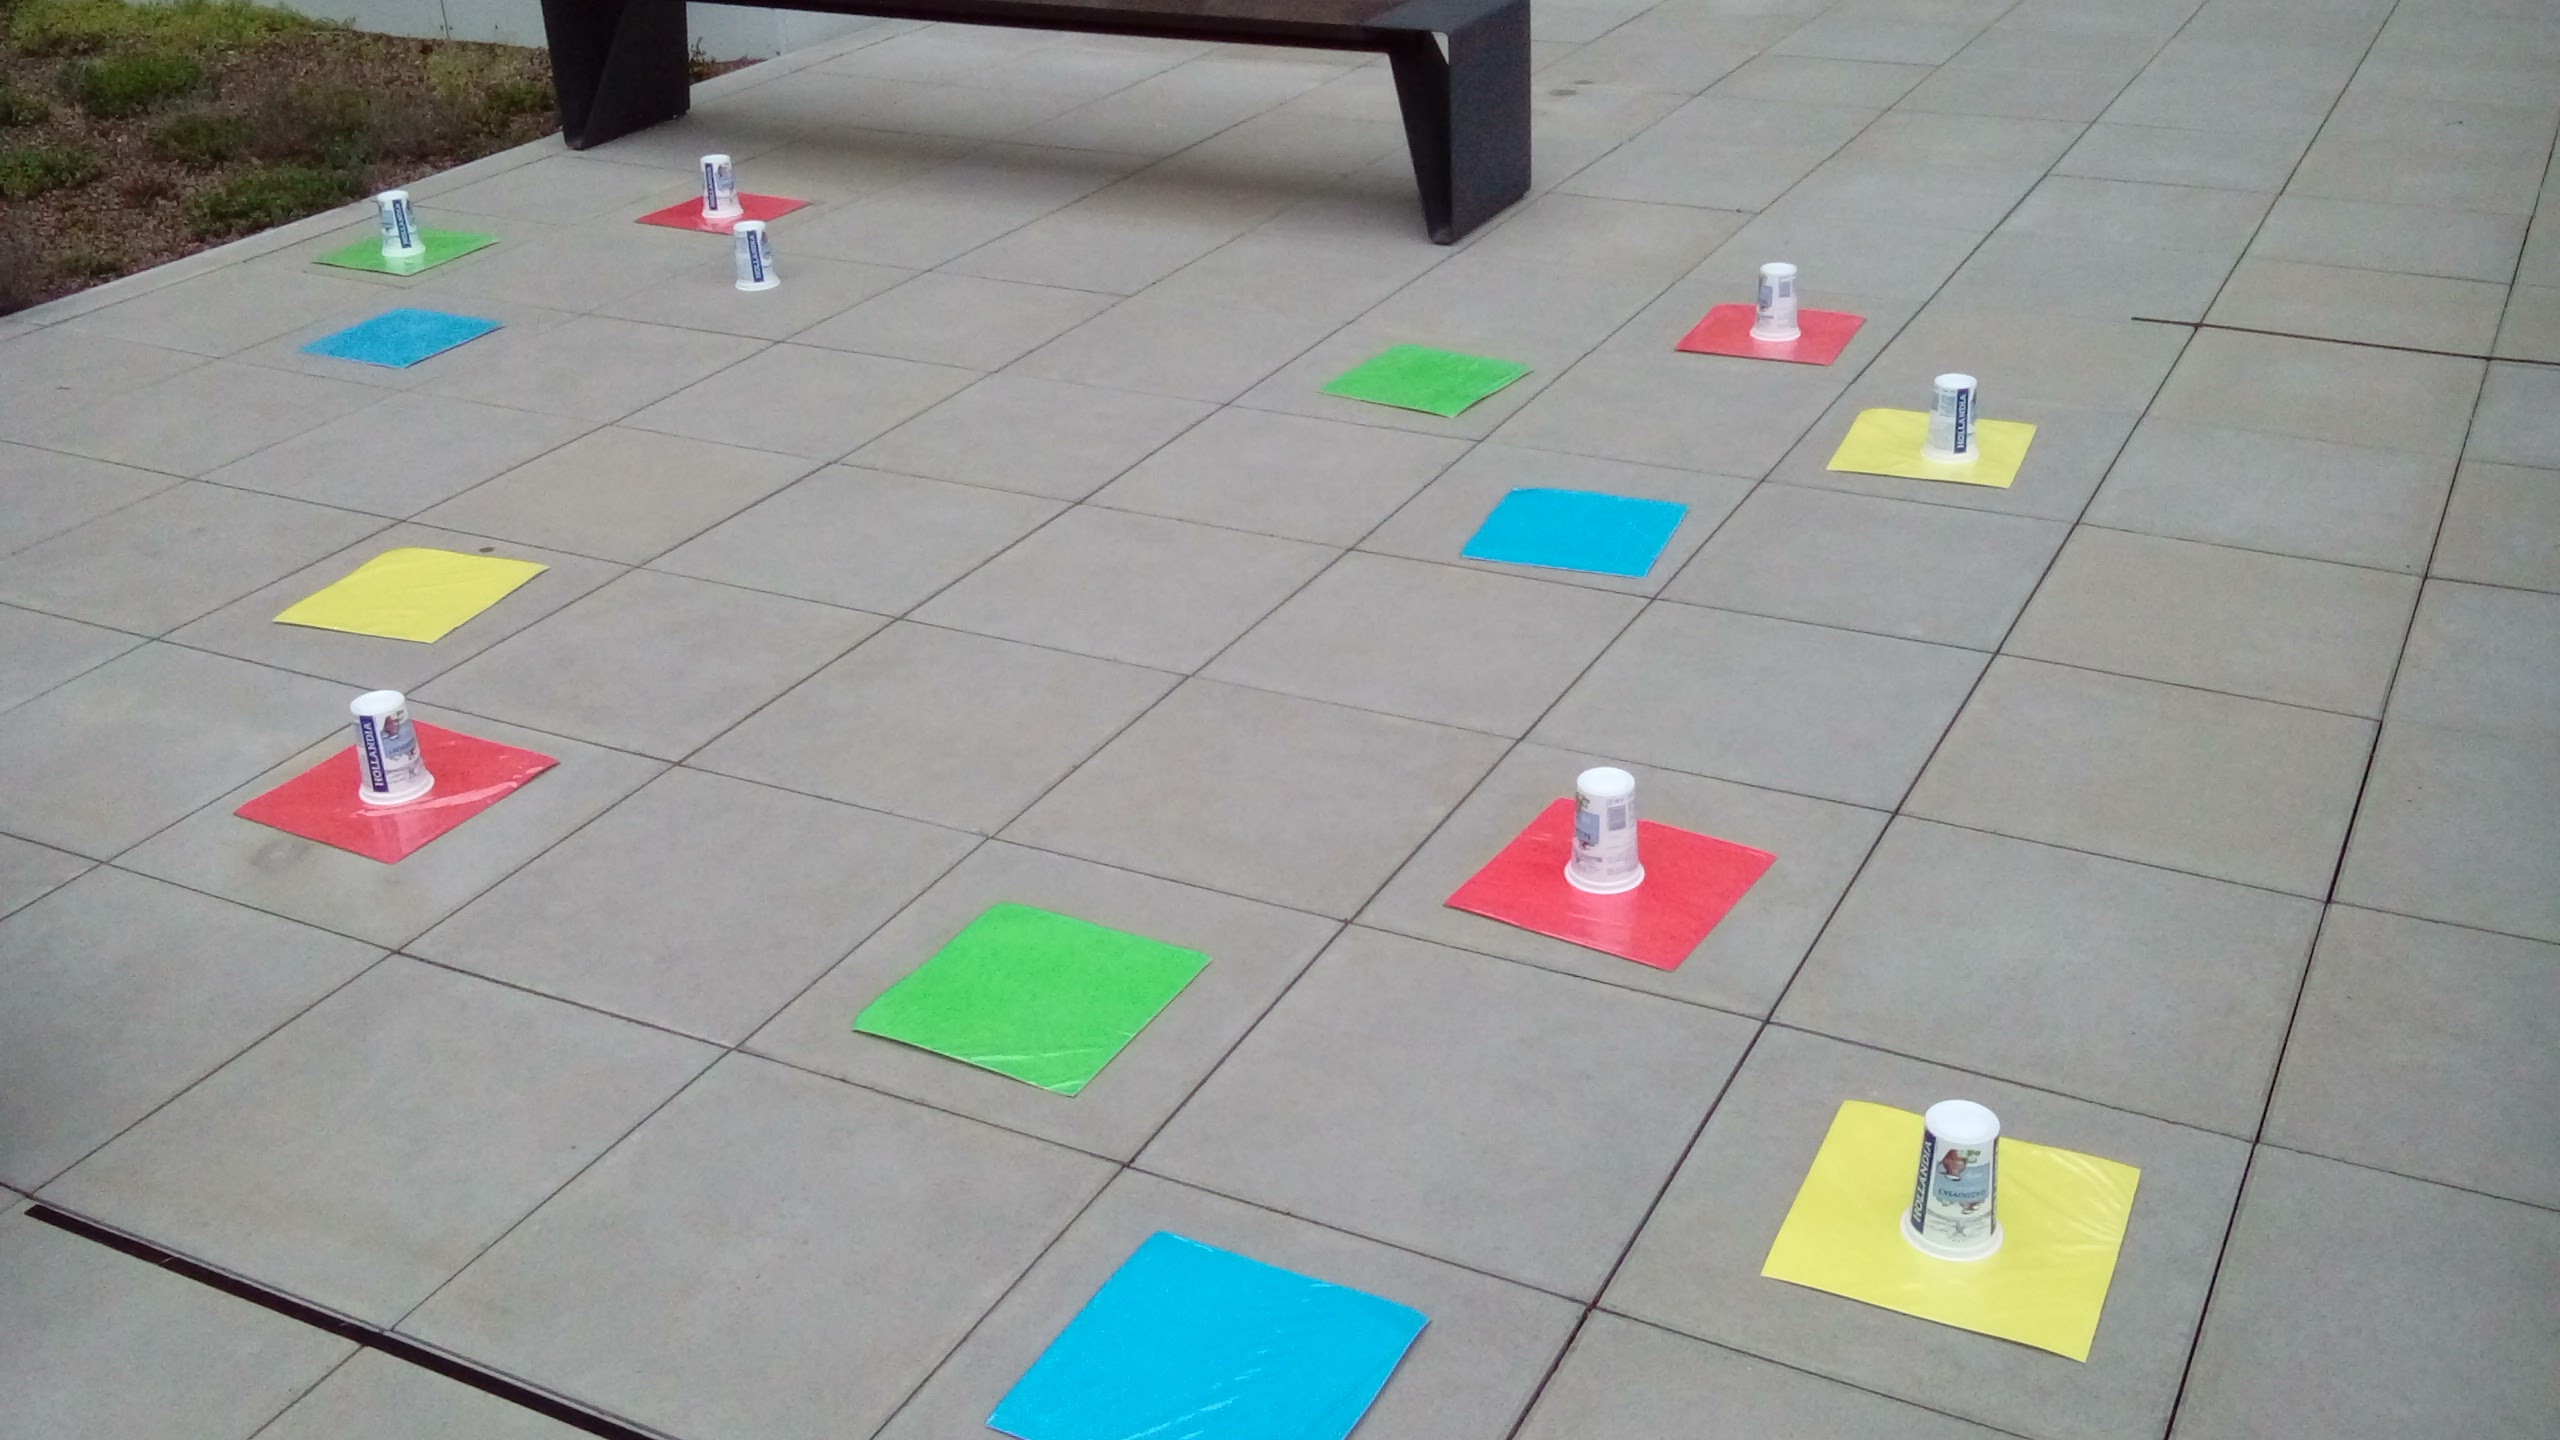
\includegraphics[width=0.65\textwidth]{img/intersob-map.jpg}\\
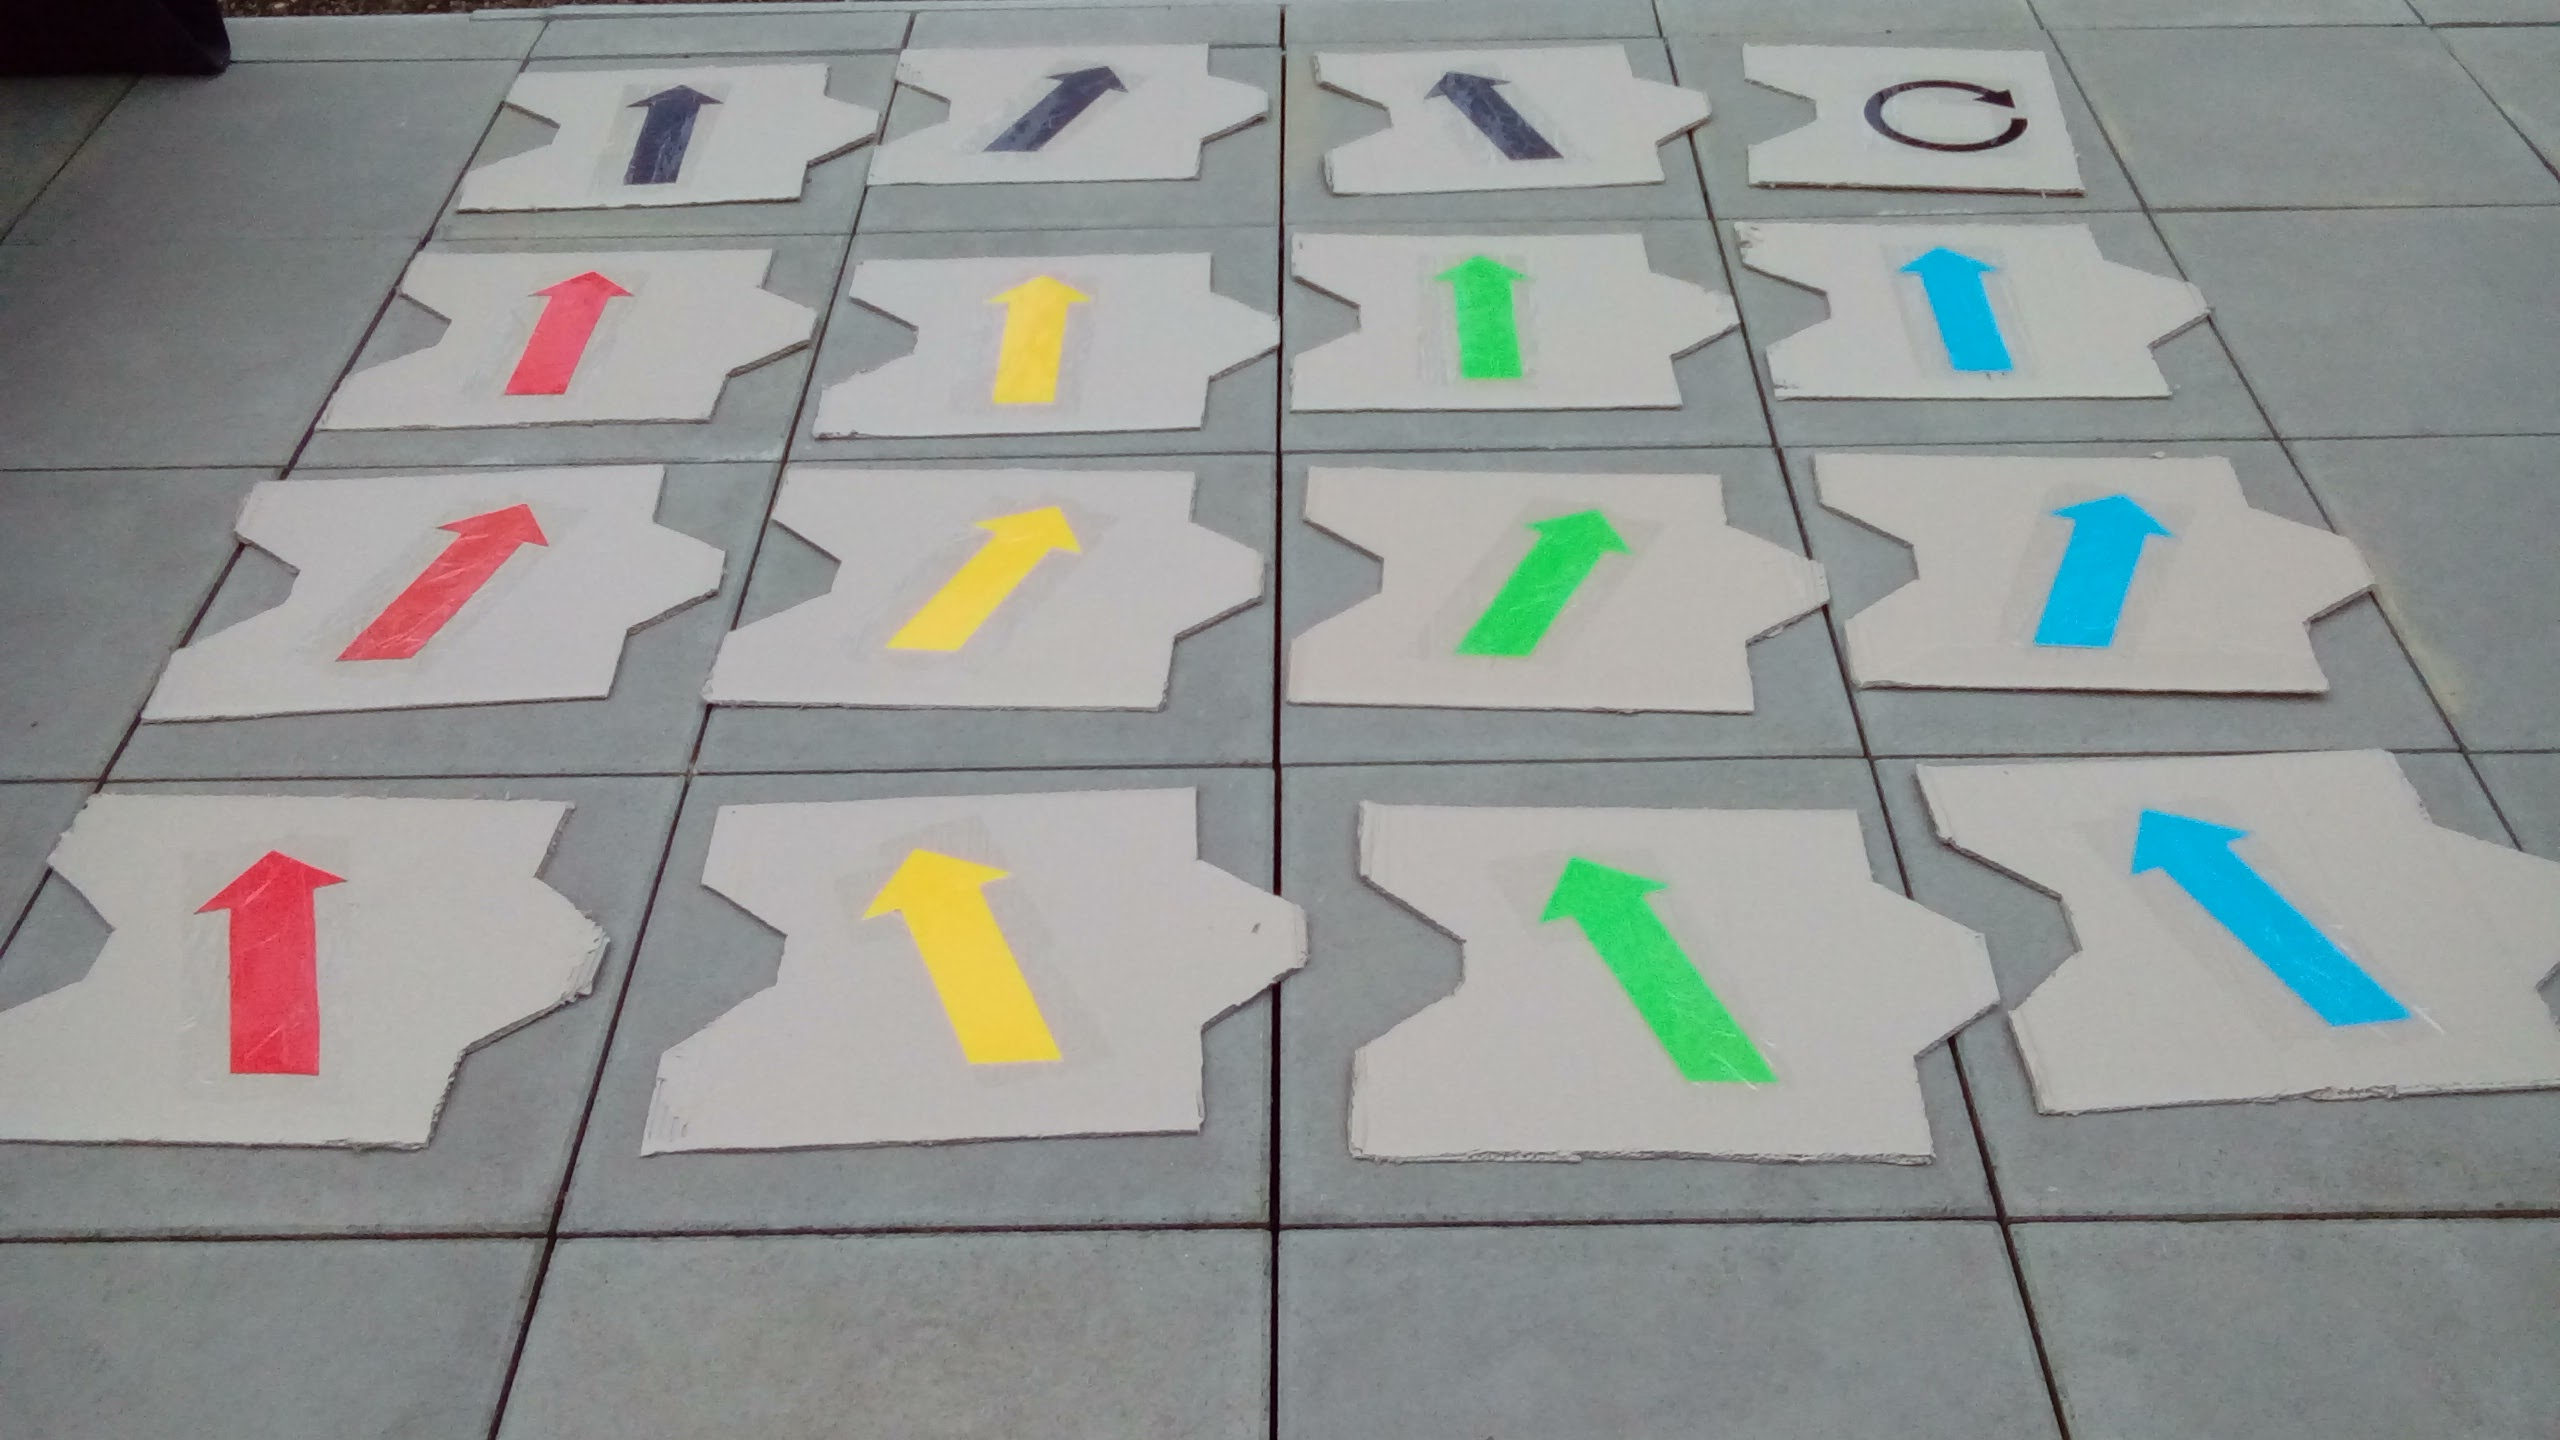
\includegraphics[width=0.65\textwidth]{img/intersob-blocks.jpg}
\end{frame}


\begin{frame}
\frametitle{Plan (2017)}
\begin{itemize}
\item feedback collection, testing on schools, data analysis $\rightarrow$ improvements
%\item promotion on schools
%\item decrease technical debt, increase robustness % refactor, test, document
\item admin, student and teacher statistics
\item new tasks, new game elements  % e.g. enemies
\item improve user interface % nicer, self-explainable, working on table/mobile
%\item complete English localization  % nearly done
\item Python-mode (for intern testing)
\end{itemize}
\end{frame}


%\begin{frame}
%\frametitle{Long Term Use Cases (2018)}
%\begin{itemize}
%% single learner mode is the only one already supported
%\item Hour of Code  % single hour,  mainly as a motivation and promotion
%\item primary school mode (RoboBlocks)  % --> teacher mode and guide
%\item secondary school mode (RoboCode)
%\item KSI -- 0th problem set % (Python)
%\item IB111 -- first motivational lesson  % --> good propagation
%\item MjUNI workshop
%\item education exhibit at VIDA  % ... Science Center
%\end{itemize}
%\end{frame}

\begin{frame}
\frametitle{Summary}
\begin{itemize}
\item system for efficient learning of programming % snaha o flow
\item grid space world, block-based programming
\item beta version:\\
  \begin{itemize}
  \item {\footnotesize \url{https://robomise.cz}}
  \end{itemize}
\item repos:\\
  \begin{itemize}
  \item {\footnotesize \url{https://github.com/adaptive-learning/flocs-web}}
  \item {\footnotesize \url{https://github.com/adaptive-learning/flocs-core}}
  \end{itemize}
\end{itemize}
\end{frame}

\end{document}
